% !TEX root = ../main.tex
\chapter{System Description}

\section{Physical Arrangement}

The apparatus is a single-axis ball and beam system. A ping-pong ball rolls along a
V-groove runner mounted on an aluminum beam. The beam pivots near the Sharp IR sensor
end and is actuated at the far end by a NEMA 17 stepper motor through a linkage. The
IR sensor measures ball distance from its sensing face, while an AS5600 magnetic sensor
measures beam angle on the actuator side.

\begin{figure}[tbp]
  \centering
  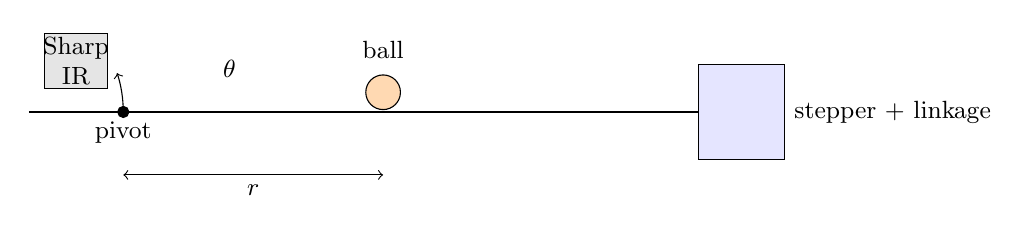
\begin{tikzpicture}[scale=1.0, every node/.style={font=\small}]
    \draw[thick] (0,0) -- (9,0);
    \filldraw[black] (1.2,0) circle (2pt);
    \node[below] at (1.2,0) {pivot};
    \draw[fill=gray!20] (0.2,0.3) rectangle (1.0,1.0);
    \node[align=center] at (0.6,0.65) {Sharp\\IR};
    \draw[fill=orange!30] (4.5,0.25) circle (0.22);
    \node[above] at (4.5,0.55) {ball};
    \draw[fill=blue!10] (8.5,-0.6) rectangle (9.6,0.6);
    \node[right] at (9.6,0) {stepper + linkage};
    \draw[<->] (1.2,-0.8) -- (4.5,-0.8);
    \node[below] at (2.85,-0.8) {$r$};
    \draw[->] (1.2,0.0) arc[start angle=0,end angle=18,radius=1.6];
    \node at (2.55,0.55) {$\theta$};
  \end{tikzpicture}
  \caption{Simplified ball and beam geometry used throughout the report. Positive
  ball position is measured away from the pivot; positive analytical beam angle raises
  the motor side.}
  \label{fig:system_geometry}
\end{figure}

\section{Coordinates and Sign Convention}

The generalized coordinates are the ball position $r$ measured from the pivot and the
beam angle $\theta$ measured from the horizontal. The analytical sign convention from
\path{modeling.md} is:

\begin{itemize}
  \item $r > 0$ means the ball is farther from the pivot and closer to the motor end.
  \item $\theta > 0$ means the motor side of the beam is up.
  \item Under this analytical convention, positive $\theta$ makes gravity pull the
  ball toward the pivot, so $r$ decreases.
\end{itemize}

The firmware uses a calibrated runtime angle \verb|theta_rel_deg| whose sign is the
opposite of the analytical small-angle model. That distinction is kept explicit in the
control chapters so the mechanics remain clean while the implementation record stays
faithful to the hardware.

\section{Measured Hardware Parameters}

Table~\ref{tab:raw_measurements} summarizes the measured geometric and inertial values
used in the model.

\begin{table}[tbp]
  \centering
  \small
  \caption{Measured hardware parameters taken from the canonical modeling record.}
  \label{tab:raw_measurements}
  \begin{tabularx}{\linewidth}{@{}l c X@{}}
    \toprule
    Quantity & Value & Notes \\
    \midrule
    Ball mass & \SI{2.8}{g} & Standard \SI{40}{mm} ping-pong ball \\
    Ball diameter & \SI{40.0}{mm} & Hollow thin-shell approximation \\
    Bare beam mass & \SI{33.2}{g} & Aluminum extrusion over \SI{263}{mm} span \\
    Sensor plus wires mass & \SI{5.3}{g} & Pivot-mounted Sharp assembly \\
    Total beam assembly mass & \SI{38.5}{g} & Beam, sensor, and wiring lumped together \\
    Beam length & \SI{263}{mm} & Clevis to clevis \\
    Sensor face from pivot & \SI{40.3}{mm} & Reference for the distance measurement \\
    Nearest usable ball distance from sensor & \SI{44.0}{mm} & Tape stop prevents foldback region \\
    Farthest usable ball distance from sensor & \SI{126.6}{mm} & Far stop in the tested runner window \\
    Stepper resolution & \num{3200} microsteps/rev & \num{200} full steps with 1/16 microstepping \\
    Rolling viscous damping & \SI{0.0125}{N.s/m} & Pre-identification estimate \\
    Pivot viscous damping & \SI{0.006}{N.m.s} & Pre-identification estimate \\
    \bottomrule
  \end{tabularx}
\end{table}

The corresponding evaluated SI parameters used later are:

\begin{itemize}
  \item ball radius $R = \SI{0.020}{m}$,
  \item ball inertia $I = \tfrac{2}{3} m R^2 = \SI{7.467e-7}{kg.m^2}$,
  \item beam assembly mass $M_b = \SI{0.0385}{kg}$,
  \item beam center of mass $L_{\text{com}} = \SI{0.11805}{m}$,
  \item beam inertia about the pivot $J = \SI{7.715e-4}{kg.m^2}$, and
  \item nominal center operating point $r_0 = \SI{0.1256}{m}$.
\end{itemize}

\section{Controller-Relevant Coordinate Translation}

The firmware record in \path{modeling.md} and \path{src/main.cpp} defines:

\begin{align}
  \theta_{\text{cal,deg}} &= 0.07666806 \cdot \theta_{\text{AS5600,deg}} - 23.28443907 \\
  \theta_{\text{rel,deg}} &= \theta_{\text{cal,deg}} - \theta_{\text{balance,deg}} \\
  x_{\text{cm}} &= d_{\text{filt,cm}} - d_{\text{setpoint,cm}}
\end{align}

with the empirically verified meanings:

\begin{itemize}
  \item $x_{\text{cm}} > 0$ means the ball is toward the motor end,
  \item manual command \verb|A+| rolls the ball toward the motor end, and
  \item near the operating point, $\theta_{\text{rel,deg}} \approx -\theta_{\text{phys,deg}}$.
\end{itemize}

This split between analytical and firmware coordinates is central to interpreting both
the model and the telemetry correctly.
